\title{Petri Nets}
\author{
        Djura Smits
}
\date{\today}

\documentclass[11pt]{article}

\usepackage[colorinlistoftodos, bordercolor=white, backgroundcolor=cyan]{todonotes}
\usepackage{pnets, graphicx}
\begin{document}
%\listoftodos
\maketitle

\section{Introduction}
Petri nets is a mathematical modeling language developed for describing distributed systems. We are considering replacing the finite state machines used in the situations framework \cite{Sung04scalablebehaviors}. Naturally, finite state automata are not directly convertible to Petri nets, so there are are a couple of issues that need to be addressed.\\
There are several aspects that we would like to have in a description of behavior:
\begin{itemize}
\item \emph{Time}\\
Since time will be the main property that we would like to improve in pedestrian simulation, it is essential that the aspect of time can be expressed in the pedestrians' behavior. Pedestrians should be able to make a decision between fulfilling their needs and reaching their (timed) goal.

\item \emph{Non-determinism}\\
In order to get varied behavior within a crowd, it is essential that the decision to make a certain behavior is stochastic, because the other option would be to define a different behavior per person, which is not feasible.

\item \emph{Availability}
Are there libraries available which we could use?

\end{itemize}

\section{Petri Nets}
A Petri net is a mathematical modeling language used for the description of distributed systems. A petri net is a bipartite graph consisting of two types of nodes: places and transitions. These nodes are connected by directed arcs. An arc can run from either a place to a transition, or from a transistion node to a place, but never from a place to a place, or between two transitions. Activity in a Petri net is expressed by by the movement of tokens from place to place, through transitions. Input arcs (from place to transition) denote which places need to contain tokens in order to enable the transition. When a transition is enabled, it consumes the tokens from the input places, and produces tokens in the place indicated by the output arc. 

\section{Advantages of Petri Nets over Finite State Automata}
Petri nets hold several advantages over finite state automata. First of all, Petri nets allow for concurrent behavior. This would enable our pedestrians to do several tasks at once. For example, it could be possible to model our pedestrians' Petri nets so that a token would represent an arm or a leg. That way, a pedestrian could execute multiple basic tasks independently. It would not be possible to achieve this kind of behavior with a finite state machine, unless a state would be described for every possible combination of activities.
However, this is not the only advantage Petri nets have over finite state automata. Petri nets come with a standardized way to incorporate a time aspect. For finite state automata, several techniques have been developed, but there is no general consensus over what methods are most suitable. The problem becomes even larger when we would like to incorporate both time and non-determinism. Both the aspects of time and non-determinism are easily incorporated in Petri nets with only small modifications, and can even be mixed with traditional Petri nets. A way to incorporate the decision of moving to the goal state or doing something else could be done by using tokens to represent time. These tokens should be used as a second input for every time-related transition. These tokens could be diminished for every unit of time, so certain transitions become inactive after a while because the time tokens that are needed for the input have run out. 
An essential issue which has to be implemented in the method we are going to choose, is non-determinism. Fortunately, this is one of the basic properties of a Petri net. When multiple transitions are enabled at the same time, any of them may fire.\\
Lastly, availability will not be an issue either, since there are many packages for many languages freely available on the web. 



\section{How Can We Replace FSMs with Petri Nets?}
While finite state automata and Petri nets look very similar, there are some essential differences which make a direct mapping impossible. First of all, Petri nets enable us to work with concurrency. This means that usually, multiple transitions are enabled in one point in time. This could mean that the pedestrian should be able to do multiple activities at once. For example, a token could be created for certain parts of the pedestrian's body, such as for its hands and feet, or upper part and lower part.\\
Another issue that has to be dealt with is how the nets are going to be attached and detached from eachother. This could be done largely the same as with finite state automata, but Petri nets have the potential to do this in a much more versatile way. For example, situation petrinets could be designed to have different slots for pedestrians so that when multiple pedestrians use the situation at the same time, the pedestrians' Petri nets could be attached to the same situation Petri net at different places, which could be a convenient way to model several kinds of behavior involving multiple pedestrians such as queueing. An example of how this could be modeled can be found in figure \ref{restaurantnet}. Customer 1 and customer 2 could be slots where a pedestrian's personal Petri net could be attached. \\
When we take an approach similar to this, there will be an important distinction between the Petri nets belonging to the pedestrians and situations. While there will be many identical pedestrian Petri nets in a simulation, there will be only one Petri net per instance of a situation. This might seem a trivial fact, but it is an important distinction between using finite state automata and Petri nets. When using finite state automata, every pedestrian will get a new instance of a situation's FSM attached to it. However, situation Petri nets will not multiply and will accept several pedestrians in their nets. This will make interaction between pedestrians in a situation a natural property of the system, in contrast to the FSM approach, where it will have to be implemented outside of the situations framework.

\begin{figure}
\caption{A simple Petri net model of a restaurant}
\begin{center}
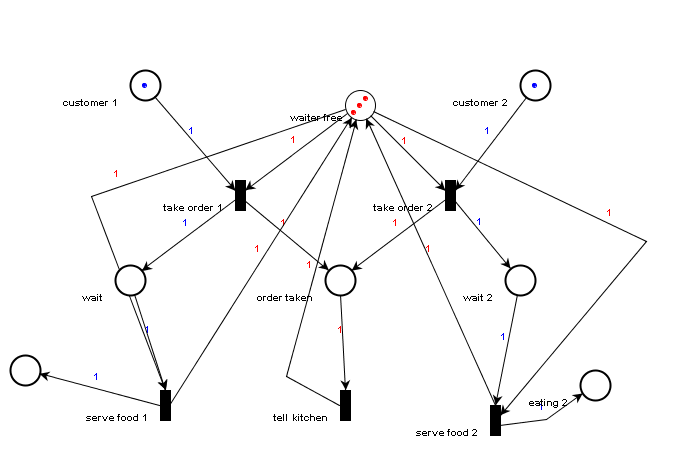
\includegraphics{restaurant}
\end{center}
\label{restaurantnet}
\end{figure}

\section{Conclusion}
We have found many advantages of Petri nets over finite state automata. It seems like Petri nets are able to support the same functionality as FSMs, but are also capable of much more, such as concurrency, and interaction between entities. This leads us to the conclusion that the situations framework could gain much from the switch of FSMs to Petri nets.

\bibliographystyle{plain}
\bibliography{references}
\end{document}
